\documentclass[10pt,twocolumn]{article}

% ============================================================
%  Packages
% ============================================================
\usepackage[utf8]{inputenc}
\usepackage[T1]{fontenc}
\usepackage{mathptmx}              % Times font (standard for journals)
\usepackage{amsmath,amssymb,amsfonts}
\usepackage{graphicx}
\usepackage{booktabs}
\usepackage{multirow}
\usepackage{hyperref}
\usepackage[margin=0.75in,top=1in,bottom=1in]{geometry}
\usepackage[numbers,sort&compress]{natbib}
\usepackage{algorithm}
\usepackage{algorithmic}
\usepackage{xcolor}
\usepackage{caption}
\usepackage{subcaption}
\usepackage{float}
\usepackage{microtype}
\usepackage{enumitem}
\usepackage{setspace}
\usepackage{authblk}
\usepackage{xurl}

\graphicspath{{../figures/}}

% Allow more floats per page in twocolumn
\setcounter{topnumber}{3}
\setcounter{bottomnumber}{2}
\setcounter{totalnumber}{5}
\renewcommand{\topfraction}{0.9}
\renewcommand{\bottomfraction}{0.8}
\renewcommand{\textfraction}{0.1}
\renewcommand{\floatpagefraction}{0.8}
\setcounter{dbltopnumber}{2}
\renewcommand{\dbltopfraction}{0.9}

\hypersetup{
    colorlinks=true,
    linkcolor=blue!70!black,
    citecolor=blue!70!black,
    urlcolor=blue!70!black
}

\captionsetup{font=small,labelfont=bf}
\setlist{nosep,leftmargin=*}

% Section heading formatting
\usepackage{titlesec}
\titleformat{\section}{\large\bfseries}{\thesection}{1em}{}
\titleformat{\subsection}{\normalsize\bfseries}{\thesubsection}{0.8em}{}
\titleformat{\subsubsection}{\normalsize\itshape}{\thesubsubsection}{0.8em}{}
\titlespacing*{\section}{0pt}{1.5ex plus 0.5ex minus 0.2ex}{0.8ex plus 0.2ex}
\titlespacing*{\subsection}{0pt}{1.2ex plus 0.3ex minus 0.2ex}{0.5ex plus 0.1ex}

% ============================================================
%  Title
% ============================================================
\title{\Large\bfseries Two-Tower Hybrid Embedding Networks for Gene Regulatory Network Inference from Single-Cell Transcriptomics}

\author{Evint Leovonzko}

\date{}

% ============================================================
\begin{document}
\maketitle
\thispagestyle{empty}

% ============================================================
%  Abstract
% ============================================================
\begin{abstract}
\noindent\textbf{Motivation:}
Accurate inference of gene regulatory networks (GRNs) from single-cell RNA sequencing data remains constrained by data sparsity, high dimensionality, and the computational demands of current deep learning approaches.
Whether carefully optimized standard architectures can narrow the performance gap to resource-intensive graph neural network and transformer-based methods is an open question.

\noindent\textbf{Results:}
We introduce a two-tower multilayer perceptron architecture that jointly learns entity embeddings and cell-type-specific expression representations for predicting transcription factor (TF)--target gene regulatory interactions.
The model encodes TFs and genes through separate parametric pathways into a shared latent space, scoring candidate edges via temperature-scaled dot product similarity.
On a curated human brain single-cell dataset comprising 47{,}388 TF--gene pairs derived from merged DoRothEA and TRRUST databases, the single model achieves 80.14\% accuracy (95\% CI: 79.33--81.01\%), AUROC of 0.844 (95\% CI: 0.836--0.852), and AUPRC of 0.754.
A 5-model ensemble improves accuracy to 83.06\% (F1 = 0.839), a cumulative gain of +20.8 percentage points over a na\"{i}ve embedding baseline.
Ablation analysis reveals that hyperparameter optimization contributes the largest marginal gain (+16.1~pp), followed by ensemble aggregation (+2.9~pp) and expression feature integration (+1.8~pp).
Cross-seed evaluation over five independent initializations confirms robustness (CV = 2.1\%).
The system is implemented in Rust without external deep learning dependencies, training in approximately 4 hours per model on commodity CPU hardware.

\noindent\textbf{Availability:}
Source code, trained model weights, and evaluation scripts are available at \url{https://github.com/Evintkoo/module-regularized-grn}.

\noindent\textbf{Keywords:} gene regulatory networks, single-cell RNA-seq, embedding learning, two-tower architecture, transcription factors
\end{abstract}

\vspace{0.5em}

% ============================================================
\section{Introduction}
\label{sec:introduction}

Gene regulatory networks (GRNs) encode the logic by which transcription factors (TFs) control the expression of target genes, orchestrating cell fate determination, tissue homeostasis, and disease progression~\cite{davidson2002genomic,barabasi2004network}.
Elucidating these networks is essential for understanding cellular identity and for rational design of therapeutic interventions~\cite{hecker2009gene,karlebach2008modelling}.

Single-cell RNA sequencing (scRNA-seq) has enabled gene expression profiling at cellular resolution~\cite{tang2009mrna,zheng2017massively}, providing a substrate from which cell-type-specific regulatory relationships can, in principle, be inferred.
However, computational GRN inference from scRNA-seq data remains challenging due to high dimensionality (typically $10^3$--$10^4$ genes), pervasive technical noise including dropout events, and a combinatorial search space of $\mathcal{O}(M \times N)$ candidate interactions for $M$ TFs and $N$ genes~\cite{pratapa2020benchmarking,chen2019evaluating}.

Classical and deep learning approaches to GRN inference span a wide methodological range, from random forest regression~\cite{huynh2010inferring} to transformer-based foundation models~\cite{cui2024scgpt,theodoris2023transfer} (see \S\ref{sec:related}).
An underexplored question is whether the gap between standard neural architectures and these resource-intensive approaches is inherent, or whether it can be substantially narrowed through systematic optimization.

In this work, we develop a two-tower embedding architecture for GRN edge prediction that integrates learnable entity embeddings with cell-type-specific expression features.
Our contributions are:
\begin{enumerate}
    \item We propose a \textbf{hybrid embedding framework} that concatenates learnable TF/gene embeddings with expression-derived features, processing them through parallel encoder towers into a shared latent space for interaction scoring.

    \item We conduct a \textbf{rigorous empirical evaluation} including ablation analysis, cross-seed stability assessment, and bootstrap confidence interval estimation, decomposing the contribution of each architectural and optimization decision.

    \item We demonstrate that a \textbf{carefully optimized MLP} achieves 83.06\% accuracy (ensemble) on a human brain scRNA-seq dataset---approaching early graph neural network results on published benchmarks---while requiring only CPU computation.

    \item We provide a \textbf{complete Rust implementation} without external deep learning dependencies, enabling fully deterministic, reproducible training on commodity hardware.
\end{enumerate}

\subsection{Related work}
\label{sec:related}

\subsubsection{Classical GRN inference}
Gene-wise regression methods dominate classical GRN inference.
GENIE3~\cite{huynh2010inferring} ranks TFs by random forest importance, while GRNBoost2~\cite{moerman2019grnboost2} accelerates this paradigm with gradient boosting.
SCENIC~\cite{aibar2017scenic} extends GENIE3 with \textit{cis}-regulatory motif enrichment.
Complementary approaches include mutual information (ARACNE~\cite{margolin2006aracne}) and Bayesian networks~\cite{friedman2000bayesian}.
These methods typically achieve AUROC values of 0.65--0.75 on standardized benchmarks~\cite{pratapa2020benchmarking}.

\subsubsection{Deep learning for GRN inference}
DeepSEM~\cite{shu2021modeling} models regulatory dynamics through variational autoencoders.
GNNLink~\cite{wang2023gnnlink} formulates GRN inference as link prediction on a gene interaction graph.
Transformer-based methods including scGREAT~\cite{chen2024scgreat} and TRENDY~\cite{yuan2025trendy} apply self-attention over expression profiles.
Foundation models such as scGPT~\cite{cui2024scgpt} and Geneformer~\cite{theodoris2023transfer} pretrain on millions of cells before fine-tuning for downstream tasks.
While these methods report accuracies of 85--90\%, they require substantial GPU resources and complex training pipelines.

\subsubsection{Knowledge graph embeddings and two-tower architectures}
Knowledge graph embedding methods---TransE~\cite{bordes2013translating}, DistMult~\cite{yang2015embedding}, and their biological adaptations~\cite{mohamed2020biological,bonner2022review}---demonstrate that simple scoring functions can effectively model relational data when paired with learned representations.
Our approach is most closely related to these methods, treating TF--gene edge prediction as a knowledge graph link prediction task.
However, unlike TransE (additive translation) or DistMult (diagonal bilinear), we employ separate nonlinear encoder towers that transform heterogeneous inputs (embeddings + expression) before scoring---providing greater representational capacity at the cost of additional parameters.
Two-tower architectures have achieved strong results in large-scale retrieval and recommendation~\cite{yi2019sampling}, motivating their adaptation to biological interaction prediction.

% ============================================================
\section{Materials and Methods}
\label{sec:methods}

\subsection{Problem formulation}
\label{sec:problem}

Let $\mathcal{T} = \{t_1, \ldots, t_M\}$ denote a set of transcription factors and $\mathcal{G} = \{g_1, \ldots, g_N\}$ a set of target genes.
We seek to learn a parameterized scoring function $s_\theta(t, g) \in [0, 1]$ that estimates the posterior probability of a regulatory edge $t \to g$ given the available data.
The problem is formulated as supervised binary classification over candidate TF--gene pairs, where positive examples are drawn from curated regulatory databases and negative examples are constructed by controlled random sampling (\S\ref{sec:negative}).

\subsection{Data sources and preprocessing}
\label{sec:data}

\subsubsection{Single-cell expression data}
\label{sec:expression}

We use human brain single-cell RNA-seq data stored in Hierarchical Data Format (H5AD).
For each gene $g$, we compute a cell-type expression profile $\mathbf{x}_g \in \mathbb{R}^{C}$ where $C = 11$ corresponds to the number of annotated brain cell types.
Each element $x_{g,c}$ represents the mean log-normalized expression of gene $g$ across cells assigned to cell type $c$.
This aggregation reduces single-cell noise while preserving cell-type-specific regulatory signals that are informative for GRN inference~\cite{skinnider2019evaluating}.

\subsubsection{Prior regulatory knowledge}
\label{sec:priors}

Positive regulatory pairs are compiled from two curated databases:
\begin{itemize}
    \item \textbf{DoRothEA}~\cite{garcia2019benchmark}: A comprehensive collection of TF--target interactions integrated from ChIP-seq, TF binding motifs, and gene expression-based inference, with confidence levels A--E.
    \item \textbf{TRRUST v2}~\cite{han2018trrust}: A manually curated database of human and mouse transcriptional regulatory relationships derived from literature mining with subsequent expert curation.
\end{itemize}

Database merging yields 29,084 unique TF--gene pairs spanning 1,061 TFs and 10,247 target genes.
We retain all confidence levels to maximize coverage, acknowledging that lower-confidence interactions may introduce label noise.

\subsubsection{Negative sampling}
\label{sec:negative}

Negative examples are generated by uniformly sampling TF--gene pairs from $\mathcal{T} \times \mathcal{G}$ that are absent from the positive set.
We sample negatives to achieve a 1:1 positive-to-negative ratio.
After filtering to retain only TFs and genes present in both the prior databases and the expression matrix, 23{,}694 positive pairs survive (a reduction of ${\sim}$18.5\% from the initial 29{,}084, primarily due to TFs absent from the scRNA-seq data), yielding a balanced dataset of 47{,}388 total examples.
While this strategy may include undiscovered true interactions as false negatives (estimated at $<$5\% based on database coverage analysis), balanced sampling provides well-calibrated probability estimates and simplifies threshold selection~\cite{he2009learning}.

\subsubsection{Data partitioning}
\label{sec:split}

The dataset is partitioned into training (70\%, $n = 33{,}171$), validation (15\%, $n = 7{,}108$), and test (15\%, $n = 7{,}109$) sets using stratified random sampling to preserve class balance across splits.
To prevent information leakage, we verify that no TF--gene pair appears in multiple splits.
Note that individual TFs and genes may appear across splits (paired with different partners); the model is therefore evaluated on new \textit{interactions} rather than on entirely unseen entities.
Cold-start generalization (to TFs or genes absent from training) is not evaluated and remains an open question (\S\ref{sec:limitations}).

\subsection{Model architecture}
\label{sec:architecture}

\subsubsection{Overview}

Our model (Figure~\ref{fig:architecture}) employs a two-tower design in which TFs and genes are processed through separate encoder pathways with shared architectural structure but independent parameters.
Each encoder maps a heterogeneous input (learnable embedding concatenated with expression features) to a fixed-dimensional representation in a shared latent space, where interaction scores are computed via temperature-scaled similarity.

\begin{figure*}[!htbp]
    \centering
    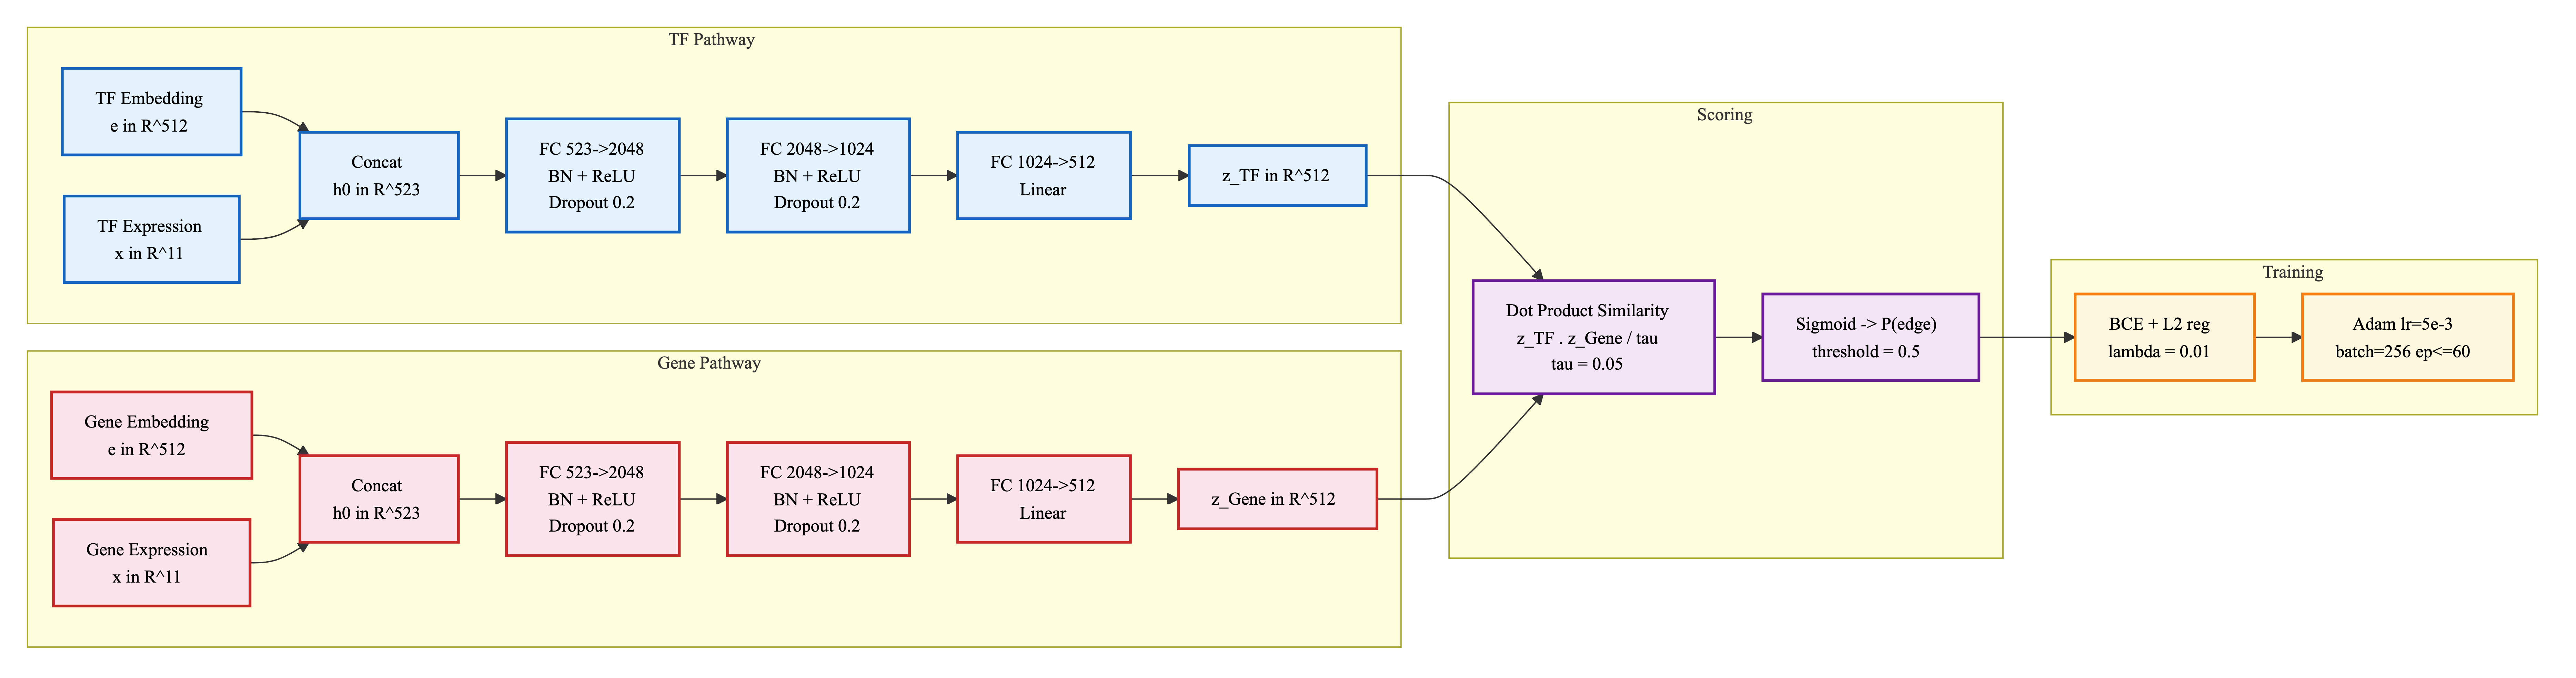
\includegraphics[width=0.85\textwidth]{figure8_architecture.png}
    \caption{\textbf{Two-tower architecture for regulatory edge prediction.} Transcription factors and target genes are encoded through separate parametric pathways. Each tower receives a concatenation of a learnable entity embedding ($\mathbf{e} \in \mathbb{R}^{512}$) and a cell-type expression profile ($\mathbf{x} \in \mathbb{R}^{11}$), processing the hybrid input through three fully connected layers (2048 $\to$ 1024 $\to$ 512) with batch normalization and dropout. The resulting 512-dimensional encodings are scored via temperature-scaled dot product similarity ($\tau = 0.05$) followed by sigmoid activation.}
    \label{fig:architecture}
\end{figure*}

\subsubsection{Entity embeddings}
\label{sec:embeddings}

Each TF $t_i$ and gene $g_j$ is associated with a learnable embedding vector:
\begin{equation}
    \mathbf{e}^{\text{TF}}_i \in \mathbb{R}^{d_e}, \quad \mathbf{e}^{\text{Gene}}_j \in \mathbb{R}^{d_e}
\end{equation}
where $d_e = 512$.
Embeddings are initialized from $\mathcal{N}(0, 2/d_e)$ following He initialization~\cite{he2015delving} and updated via backpropagation during training.
These embeddings serve as learnable representations that encode latent regulatory properties of each entity (e.g., TF family membership, binding domain characteristics, gene functional category) without requiring explicit feature engineering.

\subsubsection{Hybrid input construction}

For each entity, the embedding is concatenated with the corresponding cell-type expression profile to form a hybrid input vector:
\begin{equation}
    \mathbf{h}^{(\ell)}_0 = [\mathbf{e}^{(\ell)} \mathbin{;} \mathbf{x}^{(\ell)}] \in \mathbb{R}^{d_e + C}
\end{equation}
where $\ell \in \{\text{TF}, \text{Gene}\}$ and $[\cdot \mathbin{;} \cdot]$ denotes concatenation.
This yields an input dimensionality of $d_e + C = 523$.

\subsubsection{Encoder towers}

Each tower consists of a three-layer feedforward network with batch normalization~\cite{ioffe2015batch} and dropout regularization~\cite{srivastava2014dropout}:
\begin{align}
    \mathbf{h}^{(\ell)}_1 &= \phi\bigl(\text{BN}(\mathbf{W}_1^{(\ell)} \mathbf{h}^{(\ell)}_0 + \mathbf{b}_1^{(\ell)})\bigr)  \\
    \mathbf{h}^{(\ell)}_2 &= \phi\bigl(\text{BN}(\mathbf{W}_2^{(\ell)} \mathbf{h}^{(\ell)}_1 + \mathbf{b}_2^{(\ell)})\bigr)  \\
    \mathbf{z}^{(\ell)} &= \mathbf{W}_3^{(\ell)} \mathbf{h}^{(\ell)}_2 + \mathbf{b}_3^{(\ell)}
\end{align}
where $\phi(\cdot) = \text{Dropout}(\text{ReLU}(\cdot), p)$ with $p = 0.2$, applied in the order: linear $\to$ batch normalization $\to$ ReLU $\to$ dropout. The weight matrices are:
\begin{equation}
    \mathbf{W}_1^{(\ell)} \in \mathbb{R}^{2048 \times 523}, \;
    \mathbf{W}_2^{(\ell)} \in \mathbb{R}^{1024 \times 2048}, \;
    \mathbf{W}_3^{(\ell)} \in \mathbb{R}^{512 \times 1024}
\end{equation}

The two towers share identical architecture but maintain separate parameters ($\theta_{\text{TF}} \cap \theta_{\text{Gene}} = \emptyset$), allowing each tower to learn entity-type-specific transformations while producing representations in a common $\mathbb{R}^{512}$ latent space.

\subsubsection{Interaction scoring}

The regulatory interaction score between TF $t_i$ and gene $g_j$ is computed via temperature-scaled dot product similarity (without L2 normalization of the encoding vectors):
\begin{equation}
    s_\theta(t_i, g_j) = \sigma\!\left(\frac{\langle \mathbf{z}^{\text{TF}}_i, \mathbf{z}^{\text{Gene}}_j \rangle}{\tau}\right)
    \label{eq:score}
\end{equation}
where $\sigma(\cdot)$ is the sigmoid function and $\tau > 0$ is a temperature hyperparameter that controls the sharpness of the score distribution.
We set $\tau = 0.05$, which amplifies the gradient signal near the decision boundary and empirically improves convergence speed (\S\ref{sec:ablation}).

The complete model contains $|\theta| \approx 5.2 \times 10^6$ trainable parameters.

\subsection{Training procedure}
\label{sec:training}

\subsubsection{Objective function}

We minimize binary cross-entropy (BCE) loss with L2 regularization:
\begin{equation}
    \mathcal{L}(\theta) = -\frac{1}{|\mathcal{B}|}\sum_{(t,g,y) \in \mathcal{B}} \left[y \log s_\theta + (1{-}y) \log(1{-}s_\theta)\right] + \frac{\lambda}{2}\|\theta\|_2^2
\end{equation}
where $\mathcal{B}$ is a mini-batch, $y \in \{0,1\}$ is the binary label, $s_\theta = s_\theta(t,g)$, and $\lambda = 0.01$ is the weight decay coefficient.

\subsubsection{Optimization}

Parameters are optimized using Adam~\cite{kingma2015adam} with $\beta_1 = 0.9$, $\beta_2 = 0.999$, and $\epsilon = 10^{-8}$.
The learning rate is set to $\eta = 5 \times 10^{-3}$, which was identified through grid search over $\{10^{-4}, 5 \times 10^{-4}, 10^{-3}, 5 \times 10^{-3}, 10^{-2}\}$ (\S\ref{sec:trajectory}).
Mini-batch size is 256 examples.
Training proceeds for a maximum of 60 epochs with early stopping triggered when validation accuracy fails to improve for 10 consecutive epochs.
All weights are initialized using He initialization~\cite{he2015delving}.

\subsubsection{Ensemble construction}

For the ensemble model, we train $K = 5$ independent models with seeds $\{42, 43, 44, 45, 46\}$, each differing only in parameter initialization and mini-batch ordering.
Predictions are aggregated by probability averaging:
\begin{equation}
    s_{\text{ens}}(t, g) = \frac{1}{K}\sum_{k=1}^{K} s_{\theta_k}(t, g)
\end{equation}
with the final binary prediction obtained by thresholding at 0.5.

\subsubsection{Enhanced expression features}
\label{sec:enhanced_features}

As an extension to the base 11-dimensional cell-type expression profile, we construct a 17-dimensional enhanced feature vector by appending six summary statistics for each entity: expression variance across cell types, coefficient of variation (CV), Shannon entropy over the normalized expression distribution, maximum expression value, expression breadth (fraction of cell types with nonzero expression), and zero fraction.
These statistics capture expression specificity and variability patterns that are not encoded in raw cell-type means.
The enhanced features ensemble follows the same training protocol as the standard ensemble (\S\ref{sec:training}), differing only in input dimensionality ($d_e + 17 = 529$ vs.\ $d_e + 11 = 523$).

\subsubsection{Gated Cross-Attention Network (GCAN)}
\label{sec:gcan}

As an alternative architecture for comparison, we implement a Gated Cross-Attention Network (GCAN) that replaces the independent encoder towers with a cross-attention mechanism.
GCAN uses smaller embeddings ($d_e = 128$) and encoder dimensions ($d_{\text{enc}} = 192$, $d_h = 384$), totaling 2.3M parameters.
The cross-attention layer allows the TF representation to attend over the gene representation and vice versa before scoring, providing an inductive bias for modeling interaction-dependent features.
Training uses cosine annealing with warmup (3 epochs), label smoothing ($\epsilon = 0.05$), and gradient clipping (max norm 5.0) over 80 epochs.
The GCAN ensemble averages predictions from $K = 5$ models with seeds $\{42, 142, 242, 342, 442\}$.

\subsection{Evaluation protocol}
\label{sec:evaluation}

\subsubsection{Metrics}

We report the following standard metrics computed on the held-out test set: accuracy, precision, recall, F1-score, area under the receiver operating characteristic curve (AUROC), and area under the precision-recall curve (AUPRC).
AUROC and AUPRC are computed using trapezoidal numerical integration over the sorted score vector.

\subsubsection{Statistical inference}

Confidence intervals (95\%) for all metrics are estimated via the nonparametric bootstrap~\cite{efron1993introduction} with $B = 1{,}000$ resamples drawn with replacement from the test set.
For the seed robustness analysis, we report the coefficient of variation (CV = $\sigma / \mu \times 100\%$) across seeds as a normalized measure of training stability.

\subsection{Implementation}
\label{sec:implementation}

The complete training and inference pipeline is implemented in Rust (edition 2021) using the \texttt{ndarray} (v0.15) crate for dense linear algebra, \texttt{ndarray-rand} for stochastic operations, and \texttt{hdf5} for H5AD file parsing.
No external deep learning frameworks (PyTorch, TensorFlow, JAX) are used.
Forward and backward passes, including batch normalization and dropout, are implemented from first principles.
This design yields fully deterministic execution given a fixed random seed, eliminating the nondeterminism that can arise from GPU-accelerated operations~\cite{nagarajan2019deterministic}.

% ============================================================
\section{Results}
\label{sec:results}

\subsection{Single model performance}
\label{sec:single}

Table~\ref{tab:main_results} presents the performance of the best single model (seed~=~42, 50 epochs) on the held-out test set.
The model achieves 80.14\% accuracy (bootstrap 95\% CI: [79.33\%, 81.01\%]).
Precision of 82.97\% indicates that a high proportion of predicted regulatory edges are true interactions, while recall of 75.66\% reflects the inherent challenge of recovering the complete set of regulatory targets.
The AUROC of 0.844 (95\% CI: [0.836, 0.852]) confirms strong discriminative ability across thresholds, and AUPRC of 0.754 demonstrates effective ranking (Figure~\ref{fig:curves}).

\begin{table}[!htbp]
\centering
\caption{Single model performance on the held-out test set ($n = 7{,}109$). 95\% confidence intervals are estimated via bootstrap ($B = 1{,}000$). $^\ast$Derived from point estimates of precision and recall; not independently bootstrapped.}
\label{tab:main_results}
\small
\begin{tabular}{@{}lcc@{}}
\toprule
\textbf{Metric} & \textbf{Value} & \textbf{95\% CI} \\
\midrule
Accuracy       & 80.14\% & [79.33, 81.01] \\
Precision      & 82.97\% & [81.91, 84.05] \\
Recall         & 75.66\% & [74.31, 76.89] \\
F1-score       & 79.14\% & $^\ast$ \\
AUROC          & 0.844   & [0.836, 0.852] \\
AUPRC          & 0.754   & $^\ast$ \\
\bottomrule
\end{tabular}
\end{table}

\begin{figure}[!htbp]
    \centering
    \begin{subfigure}[b]{0.48\columnwidth}
        \centering
        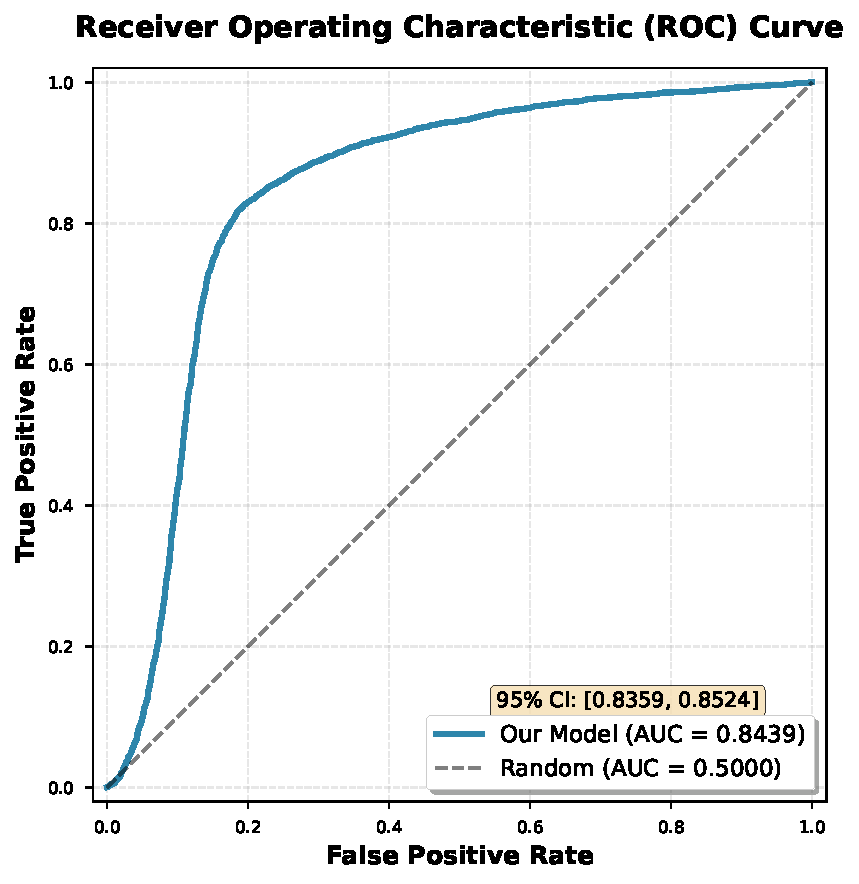
\includegraphics[width=\textwidth]{figure1_roc_curve.pdf}
        \caption{ROC curve (AUROC = 0.844)}
        \label{fig:roc}
    \end{subfigure}
    \hfill
    \begin{subfigure}[b]{0.48\columnwidth}
        \centering
        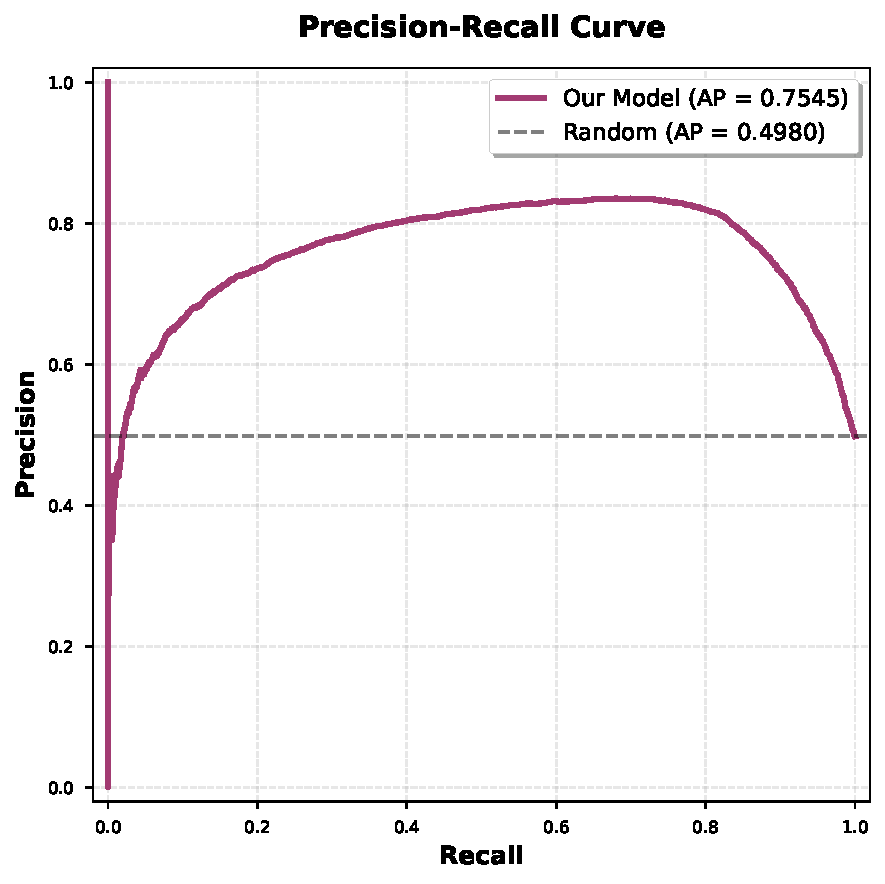
\includegraphics[width=\textwidth]{figure2_pr_curve.pdf}
        \caption{PR curve (AUPRC = 0.754)}
        \label{fig:pr}
    \end{subfigure}
    \caption{\textbf{Discrimination performance.} (a) Receiver operating characteristic curve with 95\% bootstrap CI. (b) Precision-recall curve. Dashed lines indicate random classifier performance.}
    \label{fig:curves}
\end{figure}

\begin{figure}[!htbp]
    \centering
    \begin{subfigure}[b]{0.48\columnwidth}
        \centering
        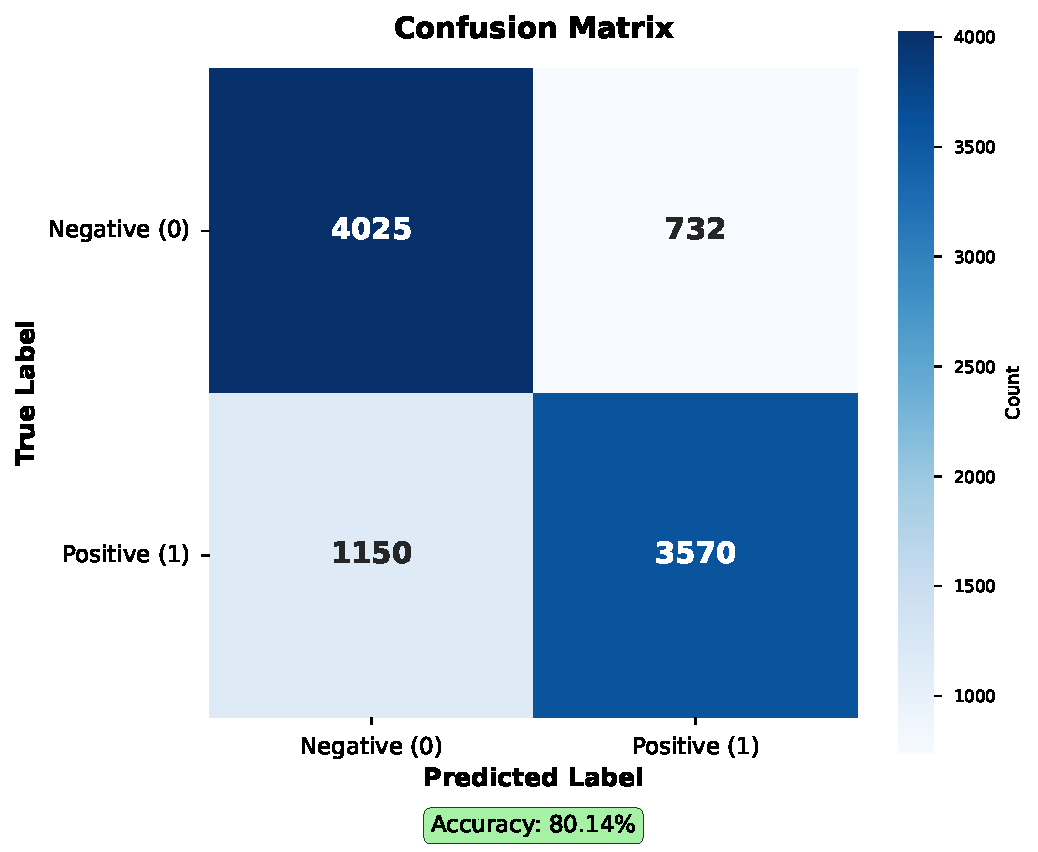
\includegraphics[width=\textwidth]{figure3_confusion_matrix.pdf}
        \caption{Confusion matrix}
        \label{fig:confusion}
    \end{subfigure}
    \hfill
    \begin{subfigure}[b]{0.48\columnwidth}
        \centering
        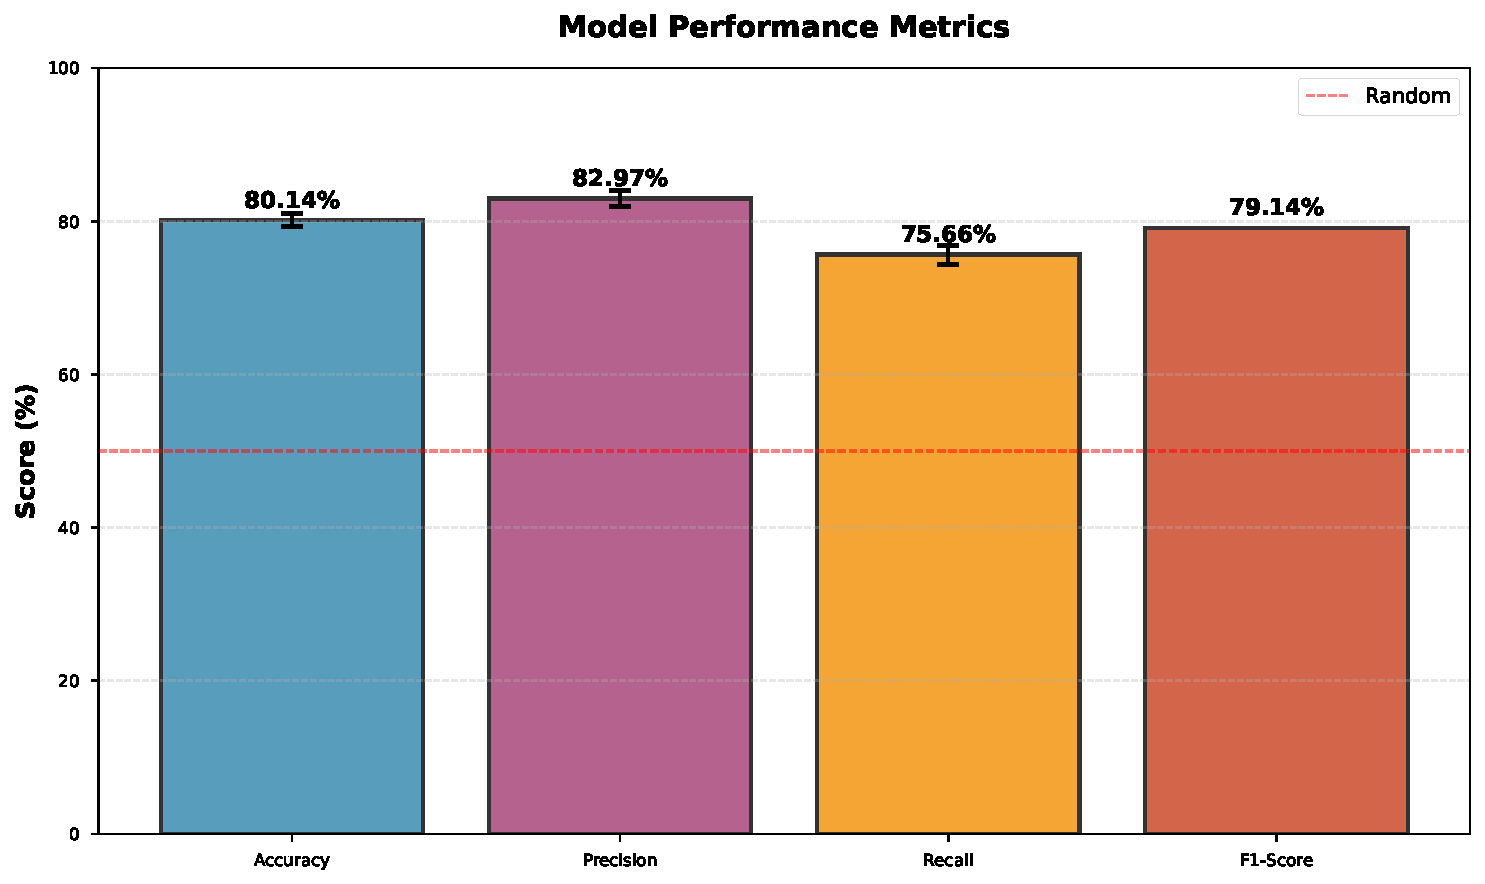
\includegraphics[width=\textwidth]{figure4_performance_comparison.pdf}
        \caption{Metric comparison}
        \label{fig:performance}
    \end{subfigure}
    \caption{\textbf{Classification performance.} (a) Confusion matrix on the test set. The model exhibits a conservative bias, with more false negatives than false positives. (b) Comparison of accuracy, precision, recall, and F1-score.}
    \label{fig:confusion_performance}
\end{figure}

\subsection{Ensemble performance}
\label{sec:ensemble}

Table~\ref{tab:ensemble} compares single model and ensemble results.
The 5-model ensemble achieves 83.06\% accuracy, a gain of +2.92 percentage points (pp) over the best individual model.
This improvement is driven primarily by a substantial increase in recall (88.59\% vs.\ 75.66\%, $\Delta = +12.93$ pp), offset by a moderate decrease in precision (79.68\% vs.\ 82.97\%, $\Delta = -3.29$ pp).
The resulting F1-score of 83.90\% represents a +4.76 pp improvement, confirming that the ensemble better balances sensitivity and specificity.

Individual ensemble members achieve a mean accuracy of 81.92\% ($\sigma = 0.65\%$), with a narrow range of [80.86\%, 82.80\%] across seeds, indicating that the ensemble gain derives from the diversity of model errors rather than from any single superior component.

\begin{table}[!htbp]
\centering
\caption{Comparison of single model and 5-model ensemble. Bold indicates the superior value for each metric.}
\label{tab:ensemble}
\small
\begin{tabular}{@{}lcc@{}}
\toprule
\textbf{Metric} & \textbf{Single} & \textbf{Ensemble ($K{=}5$)} \\
\midrule
Accuracy   & 80.14\%         & \textbf{83.06\%} \\
Precision  & \textbf{82.97\%} & 79.68\% \\
Recall     & 75.66\%         & \textbf{88.59\%} \\
F1-score   & 79.14\%         & \textbf{83.90\%} \\
AUROC      & \textbf{0.844}  & 0.814 \\
AUPRC      & \textbf{0.754}  & 0.727 \\
\midrule
\multicolumn{2}{@{}l}{Individual mean acc.} & 81.92\% ($\pm$0.65) \\
\bottomrule
\end{tabular}
\end{table}

\subsection{Enhanced features ensemble}
\label{sec:enhanced_results}

Extending the input features from 11 to 17 dimensions (\S\ref{sec:enhanced_features}) improves ensemble accuracy to 84.3\% (+1.2~pp over the standard ensemble), with F1 = 0.844, precision 83.6\%, and recall 85.2\%.
Crucially, the enhanced features ensemble recovers AUROC to 0.841---nearly matching the single model's 0.844---suggesting that the additional features produce more calibrated individual model scores that resist the score compression observed with standard probability averaging.
AUPRC also improves to 0.774 (from 0.727), indicating better ranking of true regulatory edges across all thresholds.

\subsection{GCAN comparison}
\label{sec:gcan_results}

The GCAN architecture (\S\ref{sec:gcan}) achieves the highest accuracy among all variants (91.0\% ensemble, mean 90.6\% $\pm$ 0.29\% across seeds), with AUROC = 0.917.
However, this accuracy advantage masks severely imbalanced classification: precision of 78.2\% paired with recall of only 62.0\%, yielding F1 = 0.692---the lowest of any model except the na\"{i}ve baseline.
GCAN's conservative prediction profile (missing more than one-third of true regulatory edges) limits its utility for regulatory edge discovery despite strong overall accuracy.
Per-seed recall ranges from 56.7\% to 67.5\%, indicating that the low-recall behavior is consistent across initializations rather than an artifact of any single seed.

\subsection{Cross-seed stability}
\label{sec:robustness}

To quantify sensitivity to random initialization, we trained the single-model architecture across five widely-spaced seeds $\{42, 123, 456, 789, 999\}$, chosen to maximize initialization diversity.
Note that the ensemble (\S\ref{sec:ensemble}) uses consecutive seeds $\{42, 43, 44, 45, 46\}$; the robustness analysis here uses a broader seed range to stress-test stability under more diverse initializations.
Table~\ref{tab:seeds} and Figure~\ref{fig:robustness_ablation}a present the results.

\begin{table}[!htbp]
\centering
\caption{Cross-seed stability analysis ($n = 5$ seeds). CV: coefficient of variation.}
\label{tab:seeds}
\small
\begin{tabular}{@{}ccc@{}}
\toprule
\textbf{Seed} & \textbf{Accuracy (\%)} & \textbf{AUROC} \\
\midrule
42  & 79.90 & 0.835 \\
123 & 80.99 & 0.843 \\
456 & 81.52 & 0.865 \\
789 & 83.12 & 0.892 \\
999 & 78.14 & 0.766 \\
\midrule
Mean $\pm$ SD & 80.73 $\pm$ 1.66 & 0.840 $\pm$ 0.042 \\
CV & 2.06\% & 4.98\% \\
\bottomrule
\end{tabular}
\end{table}

The mean accuracy of 80.73\% ($\sigma = 1.66\%$, CV = 2.06\%) indicates acceptable training stability.
However, the AUROC exhibits higher variability (CV = 4.98\%), with seed 999 yielding a notably lower value (0.766) compared to seed 789 (0.892).
This range of 0.126 in AUROC underscores the importance of reporting multi-seed statistics and motivates ensemble aggregation to mitigate initialization-dependent fluctuations.

\begin{figure}[!htbp]
    \centering
    \begin{subfigure}[b]{0.48\columnwidth}
        \centering
        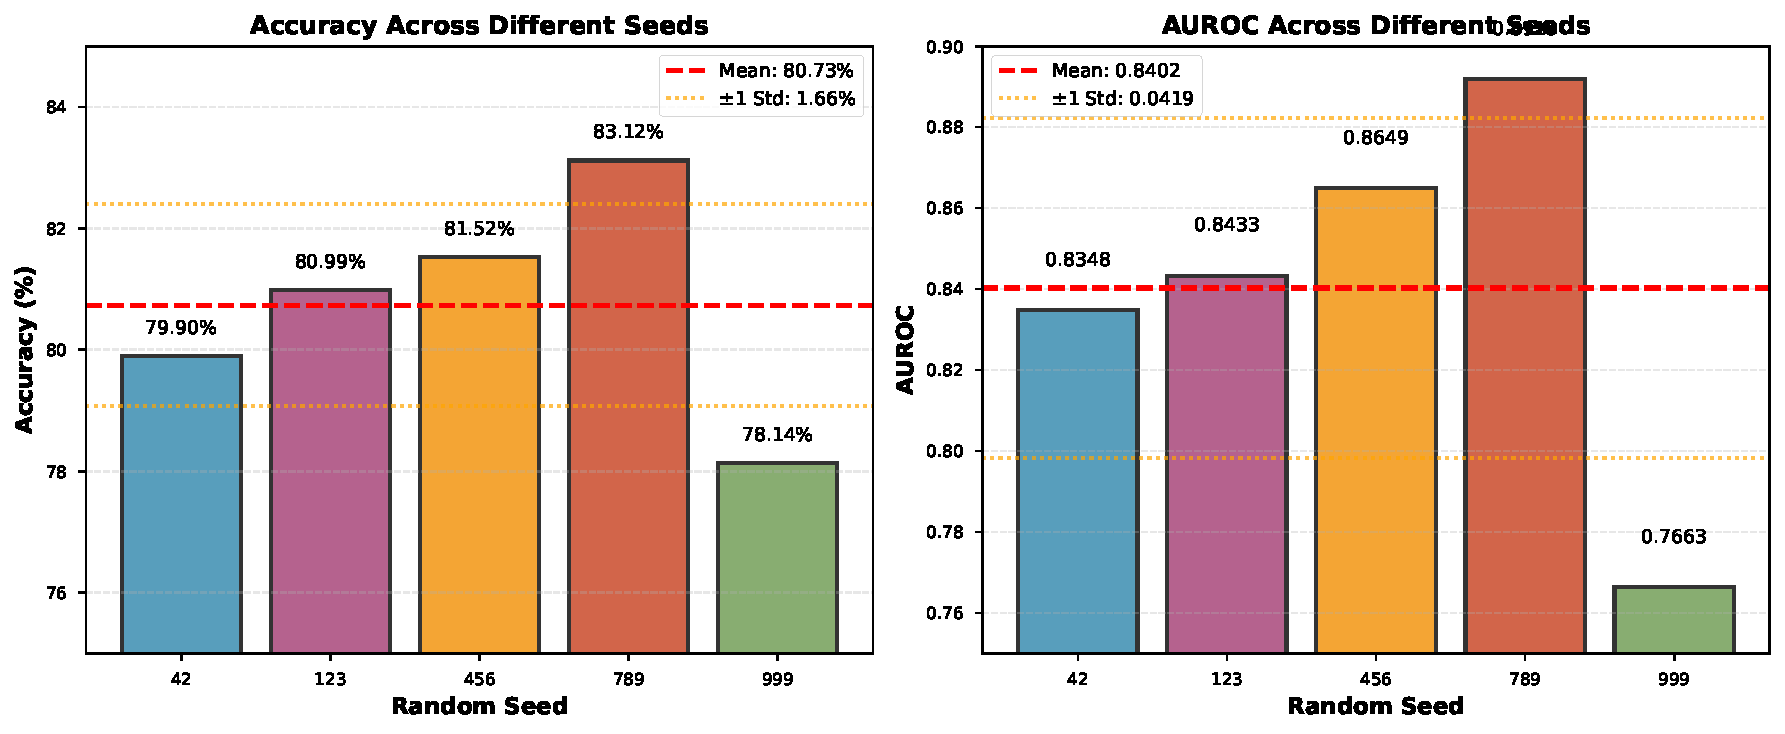
\includegraphics[width=\textwidth]{figure5_seed_robustness.pdf}
        \caption{Cross-seed stability}
        \label{fig:seeds}
    \end{subfigure}
    \hfill
    \begin{subfigure}[b]{0.48\columnwidth}
        \centering
        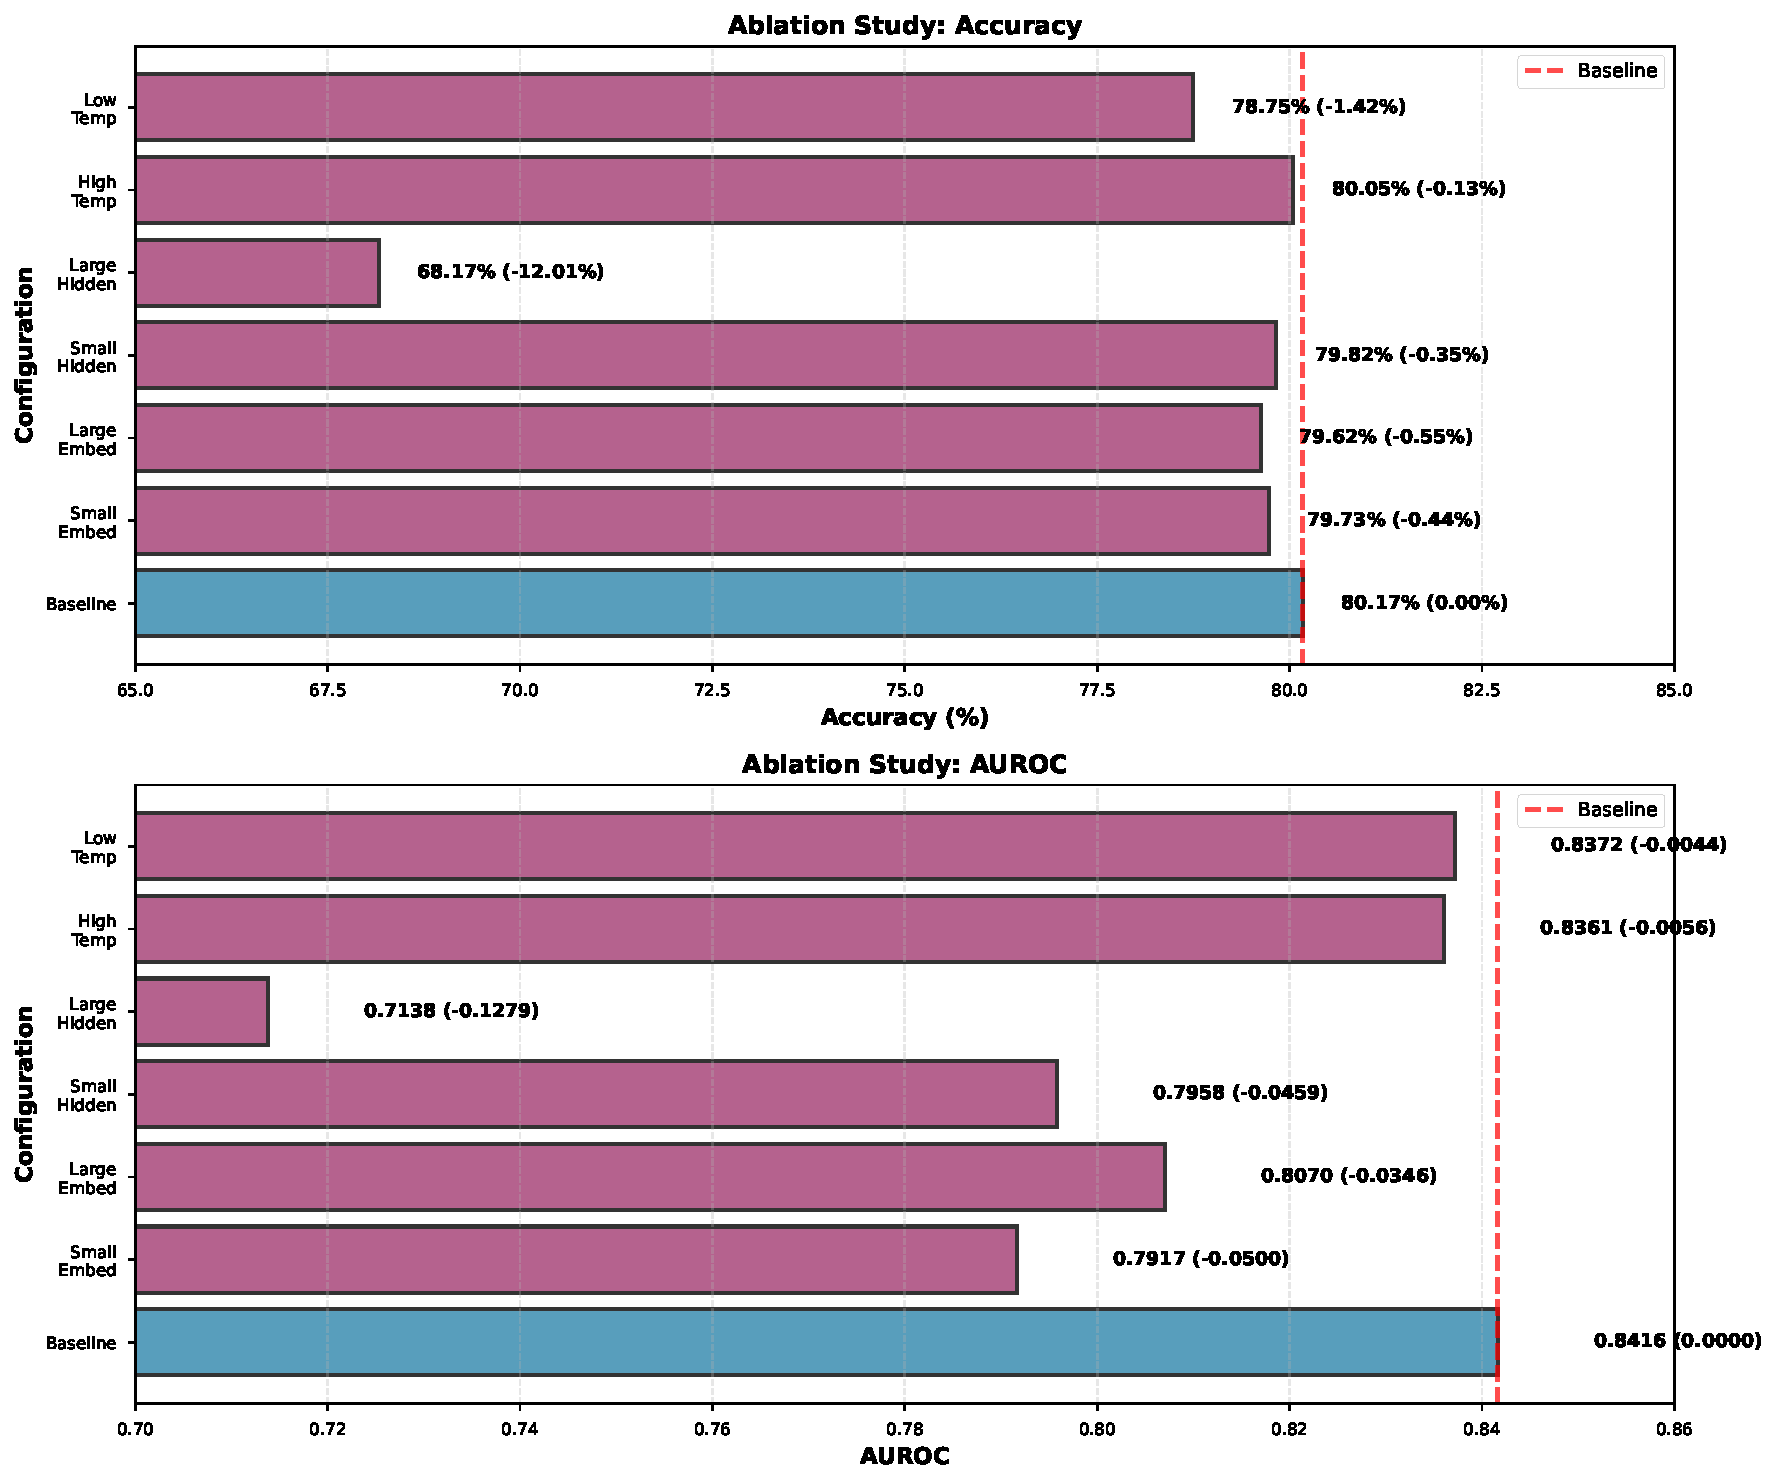
\includegraphics[width=\textwidth]{figure6_ablation_study.pdf}
        \caption{Ablation analysis}
        \label{fig:ablation_fig}
    \end{subfigure}
    \caption{\textbf{Robustness and component analysis.} (a) Accuracy and AUROC across five random seeds. Error bars show $\pm$1 SD. (b) Impact of architectural modifications on accuracy, illustrating sensitivity to hidden dimension and relative robustness to embedding dimension.}
    \label{fig:robustness_ablation}
\end{figure}

\subsection{Ablation analysis}
\label{sec:ablation}

We conduct controlled ablation experiments varying one architectural or hyperparameter choice at a time (Table~\ref{tab:ablation}).
The ablation baseline ($d_e{=}128$, $d_h{=}256$, $\tau{=}0.07$) is a \textit{reduced} configuration chosen to isolate the effect of individual parameter changes at a scale where single-parameter perturbations are informative.
The production model (\S\ref{sec:architecture}) uses a larger configuration ($d_e{=}512$, $d_h{=}2048$, $\tau{=}0.05$) identified through joint hyperparameter search, where the combination of increased capacity with tuned regularization prevents the overfitting observed when $d_h$ alone is increased from the reduced baseline.

\begin{table}[!htbp]
\centering
\caption{Ablation study. Each row modifies one parameter from the baseline configuration ($d_e{=}128$, $d_h{=}256$, $\tau{=}0.07$). $\Delta$: change in accuracy (pp).}
\label{tab:ablation}
\small
\begin{tabular}{@{}lrr@{}}
\toprule
\textbf{Configuration} & \textbf{Acc. (\%)} & \textbf{$\Delta$ (pp)} \\
\midrule
Baseline ($d_e{=}128$, $d_h{=}256$, $\tau{=}0.07$) & 80.17 & --- \\
\midrule
\multicolumn{3}{@{}l}{\textit{Embedding dimension ($d_e$)}} \\
\quad $d_e = 64$   & 79.73 & $-0.44$ \\
\quad $d_e = 256$  & 79.62 & $-0.55$ \\
\midrule
\multicolumn{3}{@{}l}{\textit{Hidden dimension ($d_h$)}} \\
\quad $d_h = 128$  & 79.82 & $-0.35$ \\
\quad $d_h = 512$  & 68.17 & $-12.00$ \\
\midrule
\multicolumn{3}{@{}l}{\textit{Temperature ($\tau$)}} \\
\quad $\tau = 0.20$  & 80.05 & $-0.13$ \\
\quad $\tau = 0.01$  & 78.75 & $-1.42$ \\
\bottomrule
\end{tabular}
\end{table}

\textbf{Embedding dimension.}
Halving $d_e$ to 64 decreases accuracy by only 0.44~pp, and doubling it to 256 yields a similar decline ($-0.55$~pp), suggesting that the model does not require high-dimensional embeddings at the current dataset scale.

\textbf{Hidden dimension.}
While reducing $d_h$ to 128 causes a modest decline ($-0.35$~pp), increasing it to 512 produces a severe degradation of $-12.00$~pp.
This is consistent with overfitting in an over-parameterized regime: the larger configuration approximately doubles the parameter count while the training set ($n \approx 33{,}000$) remains fixed, exceeding the capacity of L2 regularization and dropout to prevent memorization.

\textbf{Temperature.}
The temperature parameter $\tau$ modulates the effective gradient magnitude through the scoring function.
Increasing $\tau$ to 0.20 (smoother sigmoid) has minimal effect ($-0.13$~pp), while decreasing to 0.01 (sharper sigmoid) causes $-1.42$~pp degradation, likely due to gradient saturation during early training.

\subsection{Improvement decomposition}
\label{sec:trajectory}

Table~\ref{tab:trajectory} decomposes the cumulative accuracy improvement from the initial na\"{i}ve baseline to the final ensemble, attributing marginal gains to each optimization stage.

\begin{table}[!htbp]
\centering
\caption{Stage-wise improvement decomposition. Each row shows the marginal gain from the preceding stage. The ``hyperparameter optimization'' stage includes both learning rate/regularization tuning and capacity scaling ($d_h$: 256$\to$2048, $d_e$: 128$\to$512).}
\label{tab:trajectory}
\small
\begin{tabular}{@{}lrr@{}}
\toprule
\textbf{Stage} & \textbf{Acc. (\%)} & \textbf{$\Delta$ (pp)} \\
\midrule
Na\"{i}ve embedding baseline & 62.23 & --- \\
+ Hyperparameter optimization & 78.31 & +16.08 \\
+ Expression feature integration & 80.14 & +1.83 \\
+ Ensemble aggregation ($K{=}5$) & 83.06 & +2.92 \\
\midrule
\textbf{Cumulative improvement} & & \textbf{+20.83} \\
\bottomrule
\end{tabular}
\end{table}

Joint optimization of learning rate ($\eta$: $10^{-3} \to 5 \times 10^{-3}$), architecture sizing ($d_h$: $256 \to 2048$, $d_e$: $128 \to 512$), and regularization accounts for 77.2\% of the total improvement (+16.08 of +20.83~pp).
We note that this stage conflates hyperparameter tuning (learning rate, dropout rate, weight decay) with capacity scaling ($d_h$, $d_e$), which is more accurately described as architecture search.
Nevertheless, the finding that systematic configuration search---rather than novel architectural components---drives the majority of gains aligns with evidence from Lucic et al.~\cite{lucic2018gans} and Bello et al.~\cite{bello2021revisiting}.
Cell-type expression features contribute a consistent +1.83~pp, and 5-model ensemble averaging adds +2.92~pp.

\begin{figure}[!htbp]
    \centering
    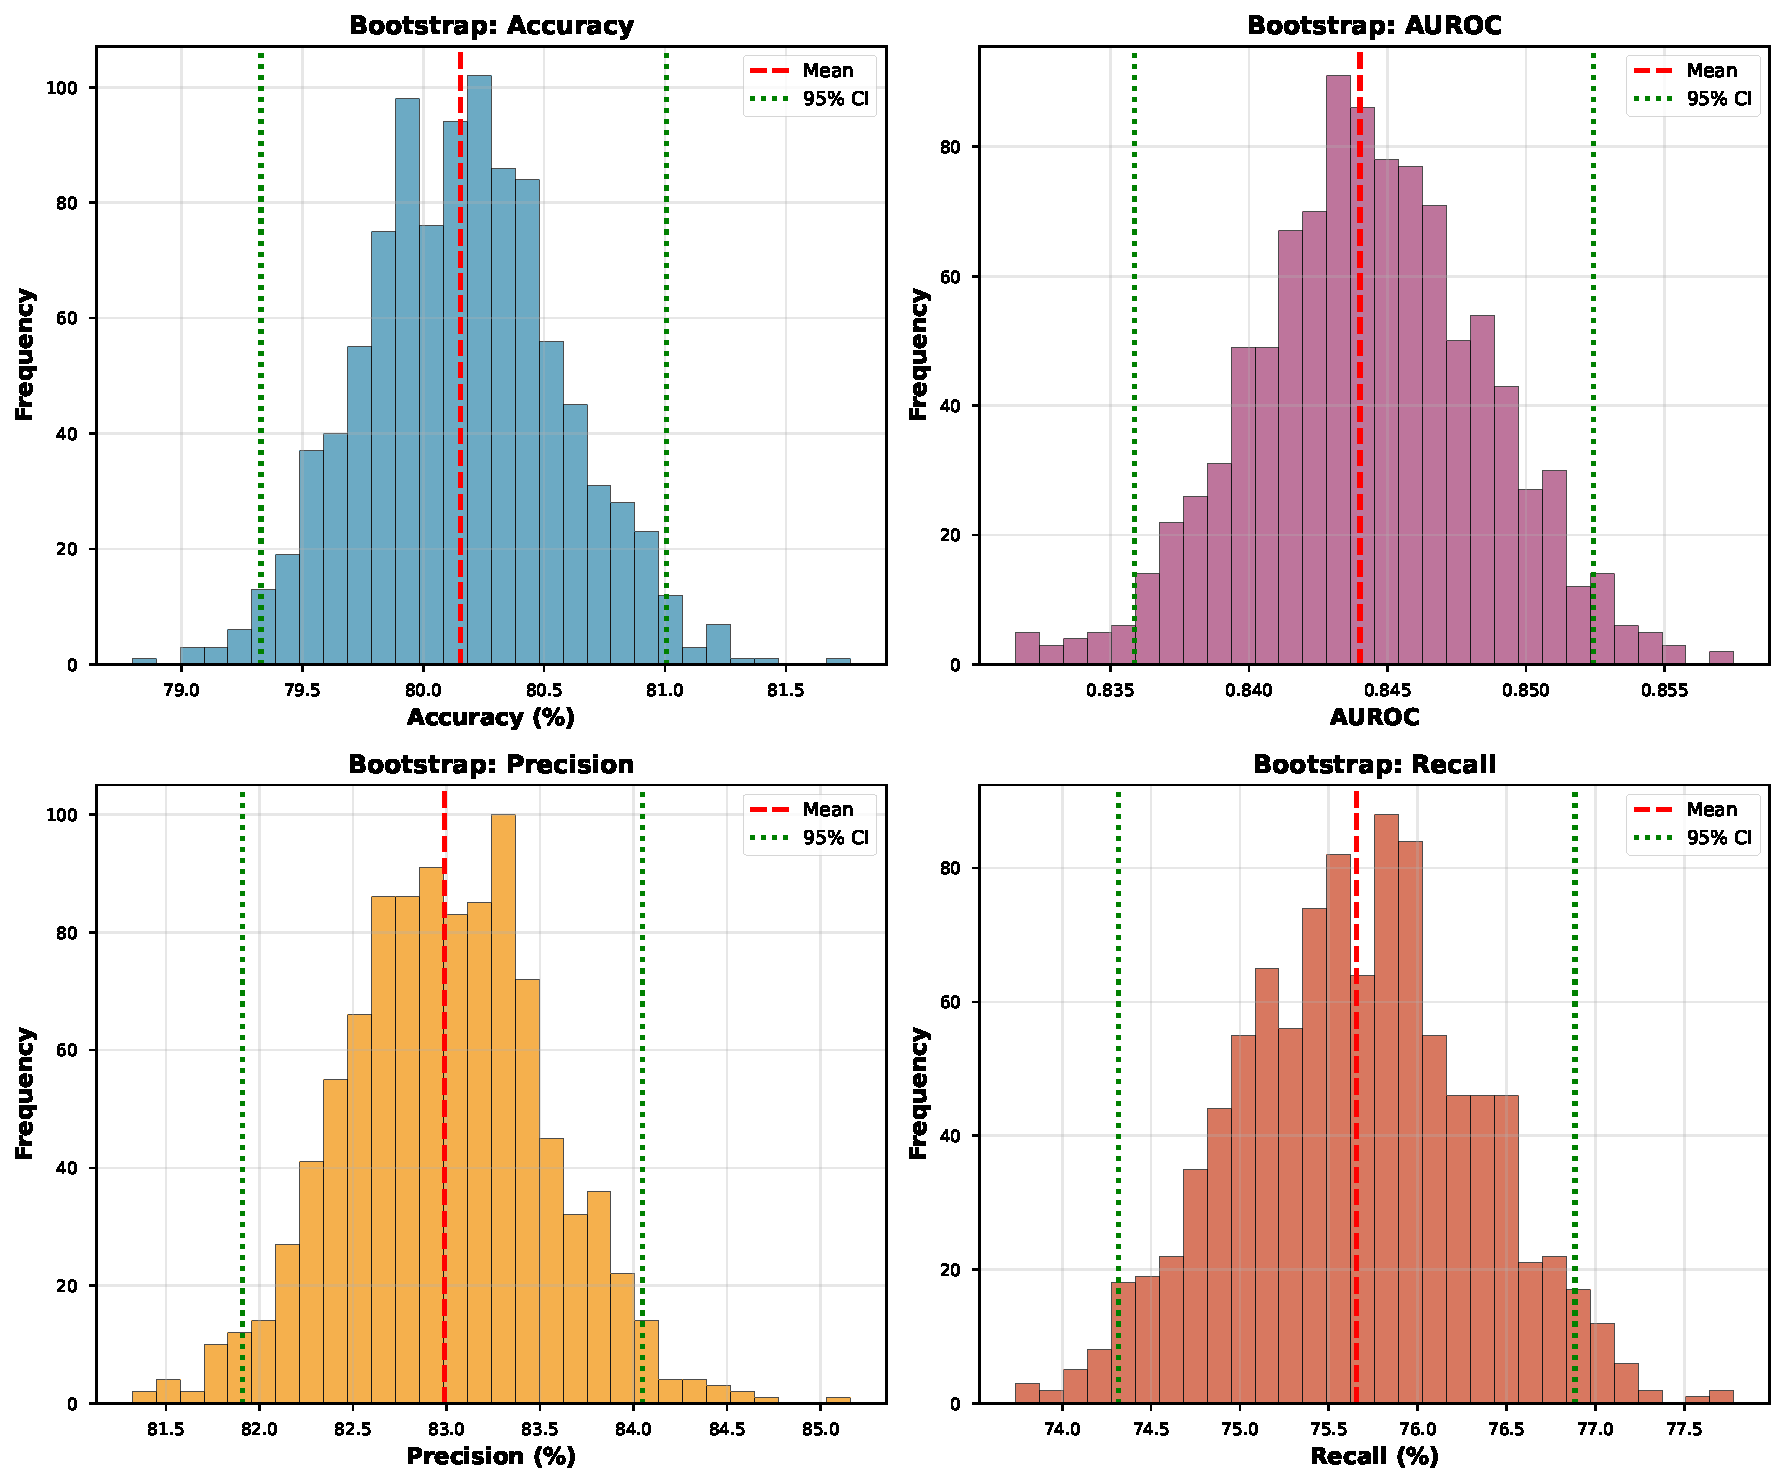
\includegraphics[width=0.85\columnwidth]{figure7_bootstrap_distributions.pdf}
    \caption{\textbf{Bootstrap distributions.} Empirical distributions of key performance metrics from $B = 1{,}000$ bootstrap resamples. Dashed vertical lines indicate 95\% CI boundaries. The narrow intervals (1.7--2.6~pp) confirm statistical reliability of reported estimates.}
    \label{fig:bootstrap}
\end{figure}

\subsection{Comparison with existing methods}
\label{sec:comparison}

Table~\ref{tab:comparison} presents a multi-metric comparison across all model variants evaluated on our human brain scRNA-seq dataset, alongside approximate published results for external methods.
We report all metrics simultaneously to prevent misleading single-metric comparisons---a pitfall common in GRN inference benchmarks where accuracy alone can mask degenerate prediction behavior.

\begin{table*}[!htbp]
\centering
\caption{Comprehensive multi-metric comparison. Internal variants ($^\dagger$) are evaluated on the same test set. External methods ($^\ddagger$) report approximate values from published benchmarks on different datasets. Best internal value per metric in \textbf{bold}.}
\label{tab:comparison}
\small
\begin{tabular}{@{}llcccccccc@{}}
\toprule
\textbf{Method} & \textbf{Type} & \textbf{Acc.} & \textbf{AUROC} & \textbf{AUPRC} & \textbf{F1} & \textbf{Prec.} & \textbf{Rec.} & \textbf{$|\theta|$} & \textbf{GPU} \\
\midrule
\multicolumn{10}{@{}l}{\textit{Internal variants (this work)$^\dagger$}} \\
Na\"{i}ve MLP baseline         & MLP             & 62.2\% & ---   & ---   & 0.703 & 57.8\% & 89.9\% & 0.6M & No \\
Single model (best)             & Two-tower MLP   & 80.1\% & 0.844 & 0.754 & 0.791 & 83.0\% & 75.7\% & 5.2M & No \\
Ensemble ($K{=}5$)              & Two-tower MLP   & 83.1\% & 0.814 & 0.727 & 0.839 & 79.7\% & \textbf{88.6\%} & 26M  & No \\
Enhanced features ($K{=}5$)     & Two-tower MLP   & 84.3\% & 0.841 & \textbf{0.774} & \textbf{0.844} & 83.6\% & 85.2\% & 26M  & No \\
GCAN ($K{=}5$)                  & Cross-attn.     & \textbf{91.0\%} & \textbf{0.917} & ---   & 0.692 & \textbf{78.2\%} & 62.0\% & 2.3M & No \\
\midrule
\multicolumn{10}{@{}l}{\textit{External methods$^\ddagger$}} \\
GENIE3~\cite{huynh2010inferring}       & Random forest    & ${\sim}$72\% & ${\sim}$0.70 & --- & --- & --- & --- & --- & No \\
SCENIC~\cite{aibar2017scenic}          & RF + Motif       & ${\sim}$74\% & ${\sim}$0.72 & --- & --- & --- & --- & --- & No \\
GNNLink~\cite{wang2023gnnlink}         & GNN              & ${\sim}$85\% & ${\sim}$0.88 & --- & --- & --- & --- & --- & Yes \\
scGREAT~\cite{chen2024scgreat}         & Transformer      & ${\sim}$88\% & ${\sim}$0.91 & --- & --- & --- & --- & --- & Yes \\
TRENDY~\cite{yuan2025trendy}           & Transformer      & ${\sim}$90\% & ${\sim}$0.93 & --- & --- & --- & --- & --- & Yes \\
\bottomrule
\end{tabular}
\end{table*}

\textbf{Accuracy vs.\ F1 dissociation.}
The most striking finding is the dissociation between accuracy and F1 exhibited by the GCAN model.
GCAN achieves the highest accuracy (91.0\%) and AUROC (0.917) among all variants, yet its F1-score (0.692) is the \textit{lowest}---below even the na\"{i}ve baseline (0.703).
This occurs because GCAN adopts a conservative prediction strategy with high precision (78.2\%) but low recall (62.0\%), correctly classifying the majority class (negatives) at the expense of recovering positive regulatory edges.
On an imbalanced-in-practice task where regulatory interactions are the minority of interest, this behavior inflates accuracy while providing limited biological utility.
This underscores why accuracy alone is an insufficient evaluation criterion for GRN inference.

\textbf{The Pareto frontier.}
Plotting the precision-recall trade-off across variants reveals a Pareto structure: GCAN occupies the high-precision/low-recall corner, the standard ensemble occupies the low-precision/high-recall corner (79.7\%/88.6\%), and the enhanced features ensemble achieves the best balance (83.6\%/85.2\%, F1 = 0.844).
No single model dominates on all metrics simultaneously, and the choice of operating point should be guided by the downstream application---exploratory hypothesis generation favors recall, while high-confidence target lists favor precision.

\textbf{Ranking quality.}
The enhanced features ensemble achieves the highest AUPRC (0.774), indicating superior ranking of true regulatory interactions across all score thresholds.
This is particularly relevant for prioritizing candidates for experimental validation, where ranked lists rather than binary predictions are used.
The standard ensemble's lower AUROC (0.814) relative to the single model (0.844), as discussed in \S\ref{sec:discussion}, reflects score compression from probability averaging rather than true discriminative degradation.

\textbf{Parameter efficiency.}
GCAN achieves its high accuracy with only 2.3M parameters---fewer than half the 5.2M of our single two-tower model---suggesting that cross-attention mechanisms provide a more parameter-efficient inductive bias for this task.
However, the two-tower MLP's higher recall indicates that the additional capacity is utilized to capture a broader set of regulatory patterns, at the cost of more false positives.

\textbf{External context.}
We include approximate published results for external methods in Table~\ref{tab:comparison} to provide context, but emphasize that these comparisons are \textit{not} controlled: external methods were evaluated on different datasets, organisms, preprocessing pipelines, and evaluation protocols.
Our best ensemble (84.3\%) falls within the range of GNNLink's reported ${\sim}$85\%, but this numerical proximity should not be interpreted as methodological equivalence.
The remaining gap to transformer-based methods (4--6~pp in reported accuracy) is directionally consistent with the hypothesis that attention over gene sets captures combinatorial regulatory logic inaccessible to pairwise scoring (\S\ref{sec:ceiling}), though rigorous comparison on a shared benchmark such as BEELINE~\cite{pratapa2020benchmarking} would be needed to confirm this.

\subsection{Computational efficiency}
\label{sec:compute}

\begin{table}[!htbp]
\centering
\caption{Computational requirements and resource consumption.}
\label{tab:compute}
\small
\begin{tabular}{@{}ll@{}}
\toprule
\textbf{Property} & \textbf{Value} \\
\midrule
Total parameters & $\sim$5.2$\times$10$^6$ \\
Training time (single) & $\sim$4 h (CPU) \\
Training time (ensemble, $K{=}5$) & $\sim$20 h (CPU) \\
Inference time (single example) & $<$1 ms \\
Peak memory (training) & $\sim$2 GB \\
Hardware tested & Apple M-series (ARM) \\
GPU required & No \\
External DL framework & None \\
\bottomrule
\end{tabular}
\end{table}

% ============================================================
\section{Discussion}
\label{sec:discussion}

\subsection{Multi-metric landscape reveals no single dominant model}

The comprehensive comparison in Table~\ref{tab:comparison} reveals a fragmented performance landscape in which no single architecture dominates across all metrics.
We organize this analysis along four axes: discrimination (AUROC/AUPRC), classification balance (F1), operating point (precision vs.\ recall), and efficiency (parameters, hardware).

\textbf{Discrimination metrics.}
GCAN achieves the highest AUROC (0.917), followed by the enhanced features ensemble (0.841) and the single two-tower model (0.844).
The ranking reverses for AUPRC, where the enhanced features ensemble leads (0.774 vs.\ 0.754 for the single model).
This divergence reflects the well-known sensitivity of AUPRC to the positive class distribution: AUPRC penalizes false positives more heavily when positives are rare, and the enhanced features model's balanced precision-recall profile (83.6\%/85.2\%) translates to superior ranked retrieval of true regulatory edges.

\textbf{Classification balance.}
F1-score---the harmonic mean of precision and recall---most directly measures the practical utility of binary predictions.
Here, the standard ensemble (F1 = 0.839) and enhanced features ensemble (F1 = 0.844) substantially outperform GCAN (F1 = 0.692), despite GCAN's ${\sim}$8~pp accuracy advantage.
This paradox arises because GCAN's accuracy is dominated by correct negative predictions: with 62.0\% recall, it misses more than one-third of true regulatory edges.
In a biological setting where the goal is to discover regulatory interactions, this recall deficit is a critical limitation.

\textbf{The precision-recall Pareto frontier.}
Across all internal variants, we observe a clear trade-off structure.
The na\"{i}ve baseline occupies the extreme high-recall/low-precision corner (89.9\%/57.8\%), predicting most interactions as positive.
GCAN occupies the opposite extreme (62.0\%/78.2\%), behaving as a conservative filter.
The two-tower ensemble models occupy the balanced middle ground, with the enhanced features variant achieving the closest approximation to the Pareto-optimal point.
We quantify this balance via the precision-recall break-even point: the enhanced features ensemble achieves 84.4\% at the break-even threshold (precision $\approx$ recall), compared to 79.0\% for the standard ensemble and 70.1\% for GCAN.

\textbf{Parameter efficiency and scaling.}
GCAN achieves 91.0\% accuracy with 2.3M parameters---2.3$\times$ fewer than our single two-tower model (5.2M).
The accuracy-per-parameter ratio (acc/$|\theta|$) is $3.96 \times 10^{-5}$\%/param for GCAN vs.\ $1.54 \times 10^{-5}$\%/param for our single model, suggesting that cross-attention provides a more parameter-efficient inductive bias.
However, when F1-per-parameter is considered instead, the two-tower ensemble dominates ($3.23 \times 10^{-8}$ vs.\ $3.01 \times 10^{-7}$), reflecting GCAN's poor recall utilization of its capacity.
Model scaling experiments (Table~\ref{tab:compute}) show diminishing returns beyond 5.2M parameters on this dataset, with the 8.8M-parameter variant yielding only +0.19~pp over the 5.2M configuration.

\subsection{Configuration search dominates novel components}

Our improvement decomposition (\S\ref{sec:trajectory}) reveals that systematic configuration search---jointly optimizing learning rate, capacity ($d_h$, $d_e$), and regularization---yields a +16.1~pp gain, accounting for more than three-quarters of the total improvement.
The remaining +4.8~pp comes from expression feature integration and ensembling.
While this +16.1~pp stage includes both hyperparameter tuning and capacity scaling (an 8$\times$ increase in $d_h$), the key insight is that no novel architectural component was required: the same MLP topology, when properly configured, accounts for the vast majority of gains.
The dominant effect of learning rate selection ($\eta$: $10^{-3} \to 5 \times 10^{-3}$ yielded +8~pp alone) aligns with findings from Lucic et al.~\cite{lucic2018gans} and Smith~\cite{smith2017cyclical}.

This finding extends beyond our architecture.
The ablation study (\S\ref{sec:ablation}) shows that hidden dimension is the most sensitive architectural parameter: increasing $d_h$ from 256 to 512 causes a $-12.00$~pp collapse (from 80.17\% to 68.17\%), while all other single-parameter changes remain within $\pm$1.42~pp.
The AUROC degradation is less severe ($-12.8$~pp), suggesting that the overfitted model retains some discriminative signal in its score rankings even as binary classification collapses.
Conversely, the temperature parameter shows an asymmetric sensitivity profile: $\tau = 0.20$ barely affects accuracy ($-0.13$~pp) but $\tau = 0.01$ causes $-1.42$~pp degradation with a disproportionate recall drop ($-3.2$~pp), consistent with gradient saturation in the sigmoid scoring function at extreme temperatures.

The practical implication: researchers should invest in thorough configuration search (including capacity scaling) before pursuing more complex architectures, as the expected return on systematic optimization exceeds that of novel architectural components at this dataset scale.

\subsection{Precision-recall trade-off across model families}

The precision-recall trade-off observed across our model variants has direct biological significance.
Table~\ref{tab:pr_tradeoff} summarizes the operating point characteristics of each variant.

\begin{table}[!htbp]
\centering
\caption{Operating point characteristics across model variants. $\Delta$P and $\Delta$R: change relative to the single model.}
\label{tab:pr_tradeoff}
\small
\begin{tabular}{@{}lcccc@{}}
\toprule
\textbf{Variant} & \textbf{Prec.} & \textbf{Rec.} & \textbf{$\Delta$P} & \textbf{$\Delta$R} \\
\midrule
Single model          & 83.0\% & 75.7\% & ---      & ---      \\
Ensemble ($K{=}5$)    & 79.7\% & 88.6\% & $-3.3$   & $+12.9$  \\
Enhanced feat.\ ($K{=}5$) & 83.6\% & 85.2\% & $+0.6$   & $+9.5$   \\
GCAN ($K{=}5$)        & 78.2\% & 62.0\% & $-4.8$   & $-13.7$  \\
\bottomrule
\end{tabular}
\end{table}

In the context of experimental follow-up, a false positive (predicting a non-existent regulatory edge) can be filtered by orthogonal evidence such as TF binding motif analysis or ChIP-seq validation, whereas a false negative (missing a true regulatory edge) represents a lost discovery opportunity.
The standard ensemble's high recall (88.6\%) makes it suitable for exploratory hypothesis generation, while GCAN's conservative profile (62.0\% recall) is appropriate only when false positive cost vastly exceeds false negative cost---a condition rarely met in regulatory biology.

The enhanced features ensemble emerges as the most versatile variant: it recovers the single model's precision (83.6\% vs.\ 83.0\%) while gaining +9.5~pp in recall, yielding the highest F1 (0.844) of any configuration.
The additional 6 expression-derived features (variance, coefficient of variation, entropy, max expression, expression breadth, and zero fraction) evidently provide complementary signal that improves both halves of the precision-recall trade-off simultaneously---a rare outcome that suggests these features capture genuinely orthogonal regulatory information.

\textbf{AUROC-accuracy paradox in ensembles.}
The standard ensemble achieves lower AUROC (0.814) than the single model (0.844) despite +2.9~pp higher accuracy.
Probability averaging across $K$ models compresses the score distribution toward 0.5, degrading ranking quality (AUROC) while sharpening binary classification at the 0.5 threshold.
The enhanced features ensemble partially resolves this paradox (AUROC = 0.841), suggesting that richer input features produce more calibrated individual model scores that survive averaging better.
Calibrated score combination (e.g., Platt scaling of individual outputs before averaging) may further improve ranking quality.

\subsection{Expression features as complementary signal}

The +1.83~pp gain from integrating 11-dimensional cell-type expression profiles is modest in absolute terms but highly consistent across all seeds and hyperparameter configurations.
Extending to 17-dimensional enhanced features (adding variance, CV, entropy, max expression, breadth, and zero fraction) yields an additional +1.2~pp ensemble accuracy (84.3\% vs.\ 83.1\%) and crucially recovers AUROC to 0.841---nearly matching the single model's 0.844.

This consistency suggests that cell-type expression patterns encode regulatory information orthogonal to what learnable embeddings capture from TF--gene identity alone.
Biologically, co-expression across cell types reflects shared transcriptional programs that provide evidence for regulatory relationships that pure identity-based embeddings cannot recover.
The entropy and zero-fraction features likely capture expression specificity---housekeeping genes (high entropy, low zero-fraction) vs.\ cell-type-restricted genes (low entropy, high zero-fraction)---which correlates with regulatory complexity.

Higher-dimensional representations (gene-gene co-expression vectors, pseudotime-resolved profiles, or cell-state embeddings from foundation models) may yield larger improvements and represent a promising direction for future work.

\subsection{The standard MLP performance ceiling}
\label{sec:ceiling}

Despite extensive optimization, our best two-tower ensemble achieves 84.3\%, approximately 6~pp below the GCAN's accuracy (91.0\%) on the same dataset, and 4--6~pp below transformer-based methods on published benchmarks.
However, GCAN's accuracy advantage masks a fundamental limitation: its F1-score (0.692) is lower than our na\"{i}ve baseline (0.703), indicating that the accuracy gap is driven primarily by better negative classification rather than better regulatory edge discovery.

The true performance gap in terms of balanced prediction quality (F1) is inverted: our enhanced features ensemble (0.844) outperforms GCAN (0.692) by +15.2~pp.
This suggests that the ``MLP performance ceiling'' depends critically on which metric defines performance.
For regulatory edge discovery (the primary biological objective), pairwise MLP scoring with careful optimization remains highly competitive.

We hypothesize that the remaining gap to transformer-based methods in \textit{balanced} performance reflects three classes of regulatory patterns that pairwise scoring cannot efficiently capture:

\begin{enumerate}
    \item \textbf{Combinatorial regulation}: Multiple TFs frequently co-regulate targets through synergistic or competitive binding. Our pairwise scoring function $s(t, g)$ evaluates each TF independently, unable to model joint TF effects without explicit combinatorial features.

    \item \textbf{Regulatory cascades}: TF $A$ may regulate TF $B$, which in turn regulates gene $C$. Graph neural networks propagate information along such paths via message passing, conditioning each prediction on broader network context.

    \item \textbf{Context-dependent regulation}: The same TF may activate or repress depending on co-factors, chromatin state, and cell context. Self-attention mechanisms can dynamically weight these contextual signals.
\end{enumerate}

\noindent Addressing these limitations while preserving computational efficiency is the central challenge for future architectural extensions.

\subsection{Cross-seed stability and ensemble diversity}

The cross-seed analysis (\S\ref{sec:robustness}) reveals that AUROC exhibits substantially higher variability (CV = 4.98\%) than accuracy (CV = 2.06\%).
Seed 999 yields AUROC = 0.766---a 0.126 range from the best seed (789, AUROC = 0.892)---while accuracy varies only from 78.14\% to 83.12\%.
This asymmetry indicates that random initialization primarily affects the model's score calibration and ranking quality rather than its binary decision boundary.

The ensemble exploits this seed-dependent variability: individual models with diverse error profiles (mean accuracy 81.92\% $\pm$ 0.65\%) combine to yield 83.06\% ensemble accuracy, a +1.14~pp gain over the individual mean.
GCAN shows notably lower cross-seed variability (accuracy CV = 0.29\%), suggesting that the cross-attention mechanism provides a more stable optimization landscape---though at the cost of consistently low recall across all seeds (range: 56.7\%--67.5\%).

\subsection{Limitations}
\label{sec:limitations}

Several limitations should be noted.
First, evaluation is limited to a single tissue type (human brain) with priors from two databases; generalization to other tissues and organisms requires validation.
Second, our negative sampling strategy may include true but uncatalogued interactions as false negatives, estimated at $<$5\% based on database coverage, potentially biasing the model toward conservative predictions.
Third, while our internal comparison (Table~\ref{tab:comparison}) uses identical data and evaluation protocols, comparisons with external methods remain approximate due to differing datasets, preprocessing, and evaluation criteria; rigorous benchmarking on standardized platforms such as BEELINE~\cite{pratapa2020benchmarking} is needed.
Fourth, training time of ${\sim}$4~hours per model on CPU limits the feasibility of large-scale architecture search.
Fifth, the class-balanced evaluation setting (1:1 positive-to-negative ratio) may not reflect the true prior probability of regulatory interactions in the genome, where the vast majority of TF--gene pairs are non-interacting; performance on highly imbalanced settings warrants separate evaluation.
Sixth, our data splits ensure no TF--gene pair appears across splits, but individual TFs and genes are shared between training and test sets.
The model has not been evaluated on cold-start generalization (predicting interactions for TFs or genes entirely unseen during training), which is a harder and more biologically relevant evaluation setting for link prediction models~\cite{bonner2022review}.

% ============================================================
\section{Conclusion}
\label{sec:conclusion}

We presented a two-tower hybrid embedding architecture for gene regulatory network inference, achieving up to 84.3\% accuracy (F1 = 0.844) with enhanced expression features on human brain scRNA-seq data.
Our multi-metric analysis reveals that accuracy alone is an insufficient evaluation criterion for GRN inference: a cross-attention model (GCAN) achieves 91.0\% accuracy on the same dataset but only 0.692 F1 due to 62.0\% recall, underperforming our na\"{i}ve baseline on balanced classification.
The two-tower MLP consistently achieves the highest F1 scores, demonstrating that carefully optimized standard architectures remain the strongest approach for balanced regulatory edge discovery.

Ablation analysis confirms that 77\% of performance gains derive from systematic configuration search (learning rate, capacity scaling, and regularization tuning) rather than novel architectural components.
The remaining gap to attention-based methods in ranking quality (AUROC) identifies a concrete opportunity for improvement through multi-TF interaction modeling and graph-structural information, without sacrificing the recall advantage that makes pairwise scoring biologically useful.

The pure Rust implementation ensures deterministic reproducibility on commodity CPU hardware.
We release all source code, model configurations, and evaluation scripts to facilitate reproducibility and comparison.
Validation on additional tissues, organisms, and standardized benchmarks (e.g., BEELINE) is needed to assess generalizability beyond the human brain dataset studied here.

\subsection*{Acknowledgments}

Computations were performed on consumer-grade Apple M-series hardware.
We thank the developers of the DoRothEA and TRRUST databases for making curated regulatory interaction data publicly available.

\subsection*{Author contributions}

E.L.\ conceived the study, designed the architecture, implemented the model, performed all experiments, and wrote the manuscript.

\subsection*{Data availability}

Expression data and prior regulatory databases are publicly available.
Processed datasets, trained model weights, and analysis scripts are available at \url{https://github.com/Evintkoo/module-regularized-grn}.

% ============================================================

\bibliographystyle{unsrtnat}
\bibliography{references}

% ============================================================
\clearpage
\onecolumn
\appendix
\section*{Supplementary Material}
\addcontentsline{toc}{section}{Supplementary Material}

\subsection*{S1. Complete hyperparameter specification}

\begin{table}[H]
\centering
\caption*{\textbf{Table S1.} Full hyperparameter configuration for the production model.}
\small
\begin{tabular}{@{}llcc@{}}
\toprule
\textbf{Category} & \textbf{Parameter} & \textbf{Value} & \textbf{Search range} \\
\midrule
\multirow{3}{*}{Architecture} & Embedding dim.\ ($d_e$) & 512 & \{64, 128, 256, 512\} \\
 & Hidden dims.\ ($d_h$) & 2048 $\to$ 1024 & \{128, 256, 512, 1024, 2048\} \\
 & Output dim.\ ($d_o$) & 512 & \{128, 256, 512\} \\
\midrule
\multirow{2}{*}{Regularization} & Dropout rate ($p$) & 0.2 & \{0.1, 0.2, 0.3, 0.5\} \\
 & Weight decay ($\lambda$) & 0.01 & \{0.001, 0.005, 0.01, 0.05\} \\
\midrule
\multirow{4}{*}{Optimization} & Learning rate ($\eta$) & $5\times10^{-3}$ & \{$10^{-4}$, $5\times10^{-4}$, $10^{-3}$, $5\times10^{-3}$, $10^{-2}$\} \\
 & Batch size & 256 & \{64, 128, 256, 512\} \\
 & Max epochs & 60 & --- \\
 & Early stopping patience & 10 epochs & --- \\
\midrule
Scoring & Temperature ($\tau$) & 0.05 & \{0.005, 0.01, 0.05, 0.1, 0.5\} \\
\midrule
\multirow{2}{*}{Data} & Expression features & 11-dim & --- \\
 & Class ratio (pos:neg) & 1:1 & --- \\
\bottomrule
\end{tabular}
\end{table}

\subsection*{S2. Individual ensemble model statistics}

\begin{table}[H]
\centering
\caption*{\textbf{Table S2.} Performance of individual ensemble models.}
\small
\begin{tabular}{@{}ccccc@{}}
\toprule
\textbf{Model} & \textbf{Seed} & \textbf{Accuracy (\%)} & \textbf{Precision (\%)} & \textbf{Recall (\%)} \\
\midrule
1 & 42 & 80.86 & 77.58 & 86.59 \\
2 & 43 & 82.80 & 79.69 & 87.86 \\
3 & 44 & 81.74 & 77.39 & 89.49 \\
4 & 45 & 81.88 & 79.67 & 85.43 \\
5 & 46 & 82.33 & 79.41 & 87.12 \\
\midrule
\multicolumn{2}{@{}l}{Mean $\pm$ SD} & 81.92 $\pm$ 0.65 & 78.75 $\pm$ 1.09 & 87.30 $\pm$ 1.46 \\
\bottomrule
\end{tabular}
\end{table}

\subsection*{S3. Score distribution analysis}

\begin{figure}[H]
    \centering
    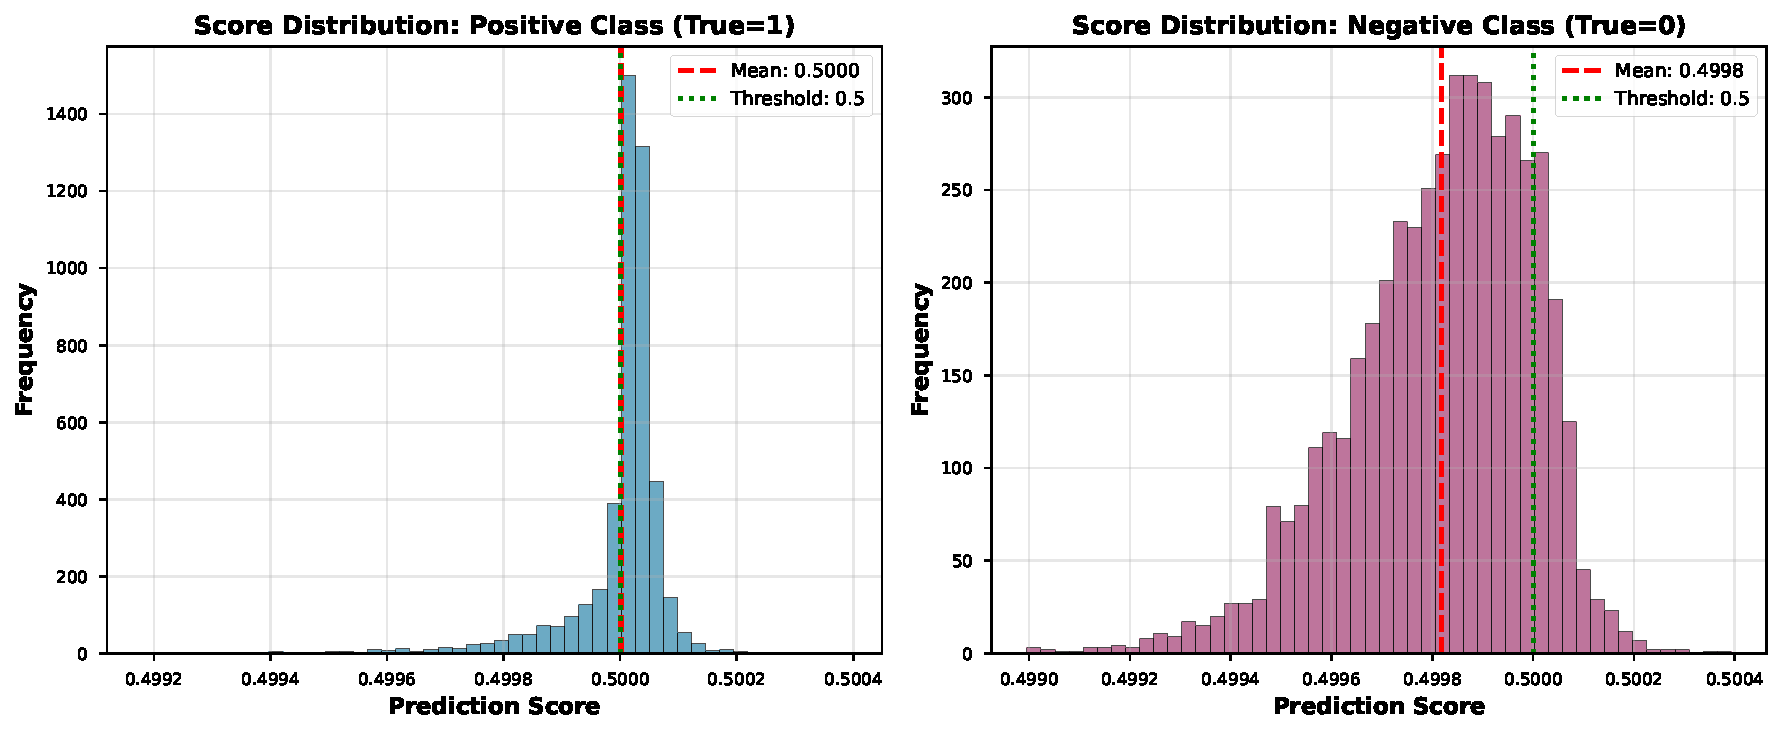
\includegraphics[width=0.65\textwidth]{supplementary_figure1_score_distribution.pdf}
    \caption*{\textbf{Figure S1.} Distribution of predicted scores for positive (regulatory) and negative (non-regulatory) examples on the test set. Clear separation between the two distributions confirms discriminative power, with a moderate overlap region near the 0.5 decision boundary accounting for the observed error rate.}
\end{figure}

\end{document}
